\begin{minipage}[t][][b]{.67\textwidth}%
	Numerical Aperture is defined as sine of largest angle that a incident ray should have for it to undergo TIR in core
	\bigskip

	By snell's law:
	$n_a\sin (\alpha)=n_1\sin (\alpha)$

	For TIR, angle of incidence	in the medium must be $>\theta_c$.

	$\alpha$ at $\theta_{c}$ is called acceptance angle. $\left(\alpha_{m}\right)$

	\begin{flalign*}
		n_a \sin \left(\alpha_{m}\right) & =n_1 \sin \left(90-\theta_{c}\right)                 &  & \\
		                                 & =n_{1} \cos (\theta)                                 &  & \\
		                                 & \equiv n_{1} \sqrt{1-\sin ^{2}(\theta_c)}            &  & \\
		                                 & =n_{1} \sqrt{1-\left(\frac{n_{2}}{n_{1}}\right)^{2}} &  & \\
		                                 & =\sqrt{n_{1}^{2}-n_{2}^{2}}                          &  &
	\end{flalign*}

	$\boxed{\therefore NA = n_{a} \cdot \sin \left(\alpha_{m}\right) =\sqrt{n_{1}^{2}-n_{2}^{2}}\ }$
\end{minipage}
\begin{minipage}[t][][b]{.3\textwidth}%
	\begin{center}
		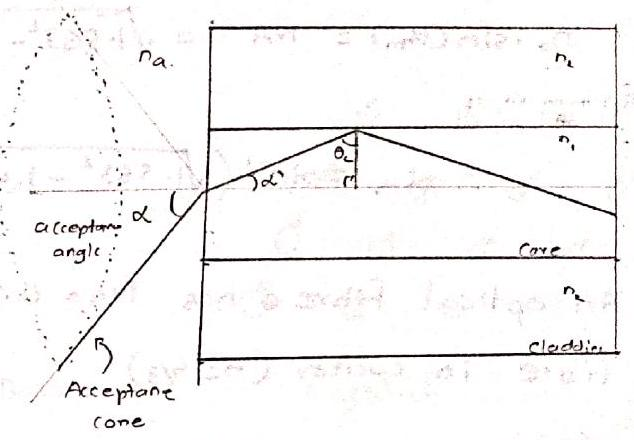
\includegraphics[max width=\textwidth]{2024_06_16_30d750483617f1939202g-06(1)}
	\end{center}

\end{minipage}
